\chapter{Visão Geral}

Para embasar e planejar o projeto a ser desenvolvido, uma proposta de
arquitetura precisa ser feito. Neste capítulo será apresentado tal proposta,
sendo inicialmente explanado a arquitetura esperada por subsistemas, e, ao fim
do capítulo, será mostrada a arquitetura geral do projeto.

\section{Subsistema - Controle e Monitoramento}

O subsistema de controle e monitoramento pode ser dividido em três grandes
componentes: a parte eletrônica da cadeira-de-rodas, um servidor remoto e um
aplicativo que será usado pelos responsáveis de um dado paciente.

A parte eletrônica será composta pelos sensores, que extraírão os sinais do
paciente, os amplificadores e filtros, que farão o tratamento do sinal
extraído, um conversor A/D, responsável por transformação dos dados tratados,
e um sistema embarcado responsável por se comunicar e enviar essas informações
para os outros componentes.

O servidor remoto será um servidor hospedado fora da rede-interna da parte
eletrônica, e poderá ser acessado via \textit{internet}. Se comunicará com
o sistema embarcado da parte eletrônica utilizando comunicação
\textit{via socket}\footnote{\url{https://docs.oracle.com/javase/tutorial/networking/sockets/definition.html}},
apresentará dados ao aplicativo, e o notificará de ocorrência de eventos
críticos.

O aplicativo, que será utilizado pelos responsáveis do paciente, estará
preparado para receber as notificações do servidor e para mostrar os dados em
tempo real.

Abaixo é possível ver o ciclo-de-vida típico do subsistema.

\begin{figure}[H]
  \centering
    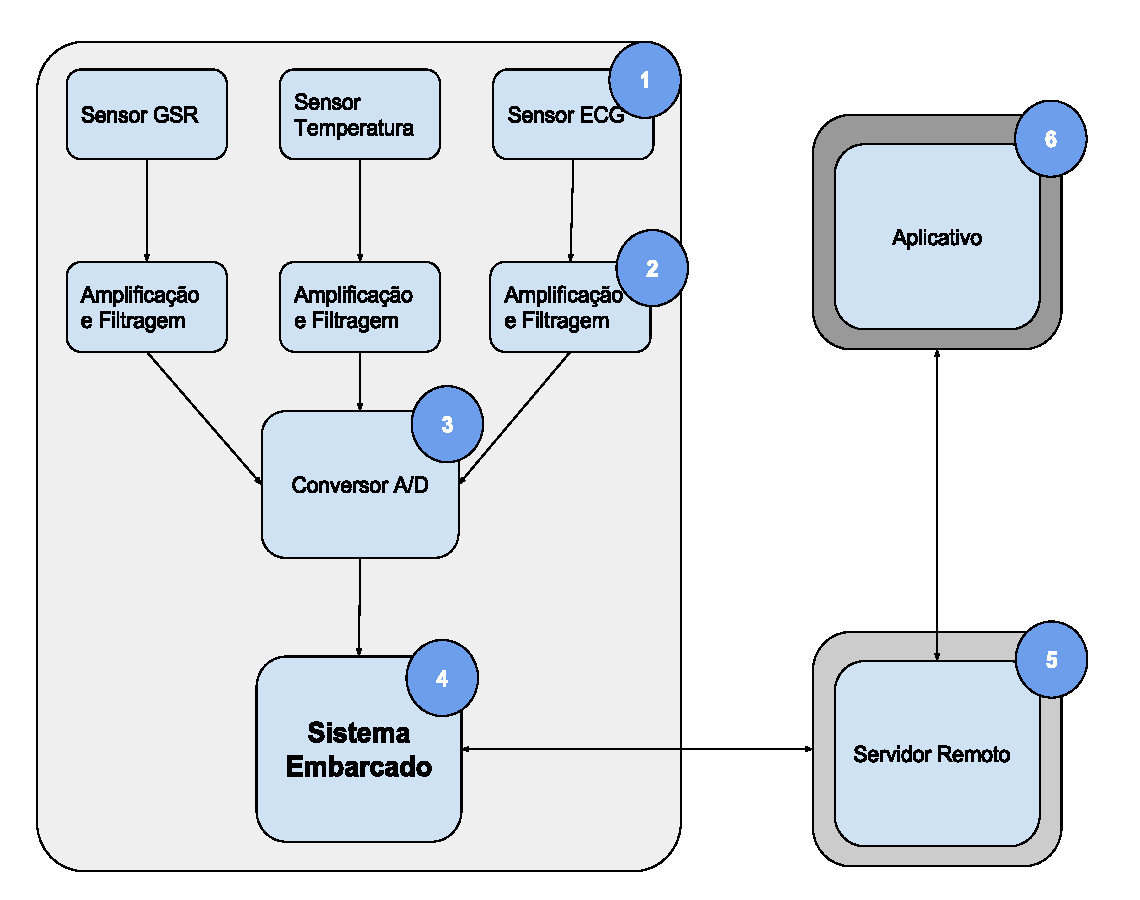
\includegraphics[width=\textwidth]{figuras/arquitetura-monitoramentoecontrole.eps}
  \caption{Fluxo típico do subsistema de Monitoramento e Controle}
  \label{fig:arquitetura-monitoramento-e-controle}
\end{figure}

O passo (1) do subsistema é atuado pelos sensores, que extraírão sinais do paciente;
o passo (2) será atuado pelos amplificadores e filtros, e tratarão o sinal
extraído pelos sensores no passo anterior; no passo (3) os sinais tratados
são convertidos para formato digital, para que possam ser lidos pelo sistema
embarcado; no passo (4) o sistema embarcado recebe as informações do conversor
e abre conexão com o servidor remoto - após, envia as informações recebidas,
quando necessário; no passo (5) o servidor remoto recebe dados do sistema
embarcado e passa informações importantes para o aplicativo, e, por fim,
no passo (6), o aplicativo recebe as informações.

\subsection{Tecnologias Utilizadas}

\section{Subsistema - Alimentação}

\section{Subsistema - Estrutura}

\section{Outros}

\subsection{Integração Contínua}
